\section{Confronto prestazionale tra l'algoritmo naive e HK76}
Il confronto prestazionale (dal punto di vista temporale) tra l'algoritmo di Hoshen-Kopelman (\textit{blu}) e quello di etichettatura naive (\textit{arancione}), precedentemente implementato, è stato condotto attraverso due diverse analisi: la prima ha considerato il tempo di calcolo richiesto per l'esecuzione degli algoritmi mantenendo costante la probabilità di colorazione dei siti e variando la dimensione del reticolo; la seconda, invece, ha analizzato il tempo di calcolo mantenendo costante la dimensione del reticolo e variando la probabilità di colorazione dei siti.

\begin{figure}
	\centering
	\includegraphics[width=0.85\linewidth]{images/compare\_t}
	\caption{Tempo di esecuzione in funzione della dimensione del reticolo per gli algoritmi HK76 e naive.}
	\label{fig:comparet}
\end{figure}
\subsection{Confronto con probabilità costante e taglia variabile}
Nel primo caso è stata fissata una probabilità di colorazione dei siti pari al $60\%$, variando la dimensione del reticolo quadrato nell'intervallo compreso tra $100$ e $1000$, con incrementi di $100$, per un totale di $10$ configurazioni. La Figura~\ref{fig:comparet} mostra i tempi medi di esecuzione degli algoritmi, calcolati eseguendo ciascuna configurazione per 50 volte. Si osservi come, all’aumentare della dimensione del reticolo, l’algoritmo HK76 offra prestazioni temporali migliori rispetto all’algoritmo naive. Di seguito sono riportati i tempi medi di esecuzione:

\vspace{15px}
\noindent
\begin{tabular}{|c|*{10}{c|}}
	\hline
	\textbf{hk76} &0.0005 &	0.0018 &	0.0037 &	0.0065 &	0.0099 &	0.0140 &	0.0192 &	0.0255 &	0.0313 &	0.0385 \\
	\hline
	\textbf{naive} & 0.0023  &  0.0090  &  0.0199 &   0.0354 &   0.0552  &  0.0806 &   0.1097  &  0.1482 &   0.1877  &  0.2383\\
	\hline
\end{tabular}
\newpage
\noindent
e i relativi errori (da moltiplicare per $10^{-3}$):

\vspace{15px}
\noindent
\begin{tabular}{|c|*{10}{c|}}
	\hline
	\textbf{hk76}  & 0.0107  &  0.0511    &0.0261 &   0.0830   & 0.1095   & 0.1083  &  0.1271  &  0.1536  &  0.1598  &  0.1649\\
	\hline
	\textbf{naive}  &0.0108  &  0.0224  &  0.0177  &  0.1090  &  0.1216  &  0.2112   & 0.2641  &  0.2072&    0.3270  &  0.4488\\
	\hline
\end{tabular}

\subsection{Confronto con taglia costante e probabilità variabile}
Nel secondo caso, invece, la dimensione del reticolo è stata mantenuta fissa a $500$, mentre la probabilità di colorazione dei siti è stata variata da $0.1$ a $1$, con incrementi di $0.1$, per un totale di $10$ esperimenti. 

\begin{figure}[H]
	\centering
	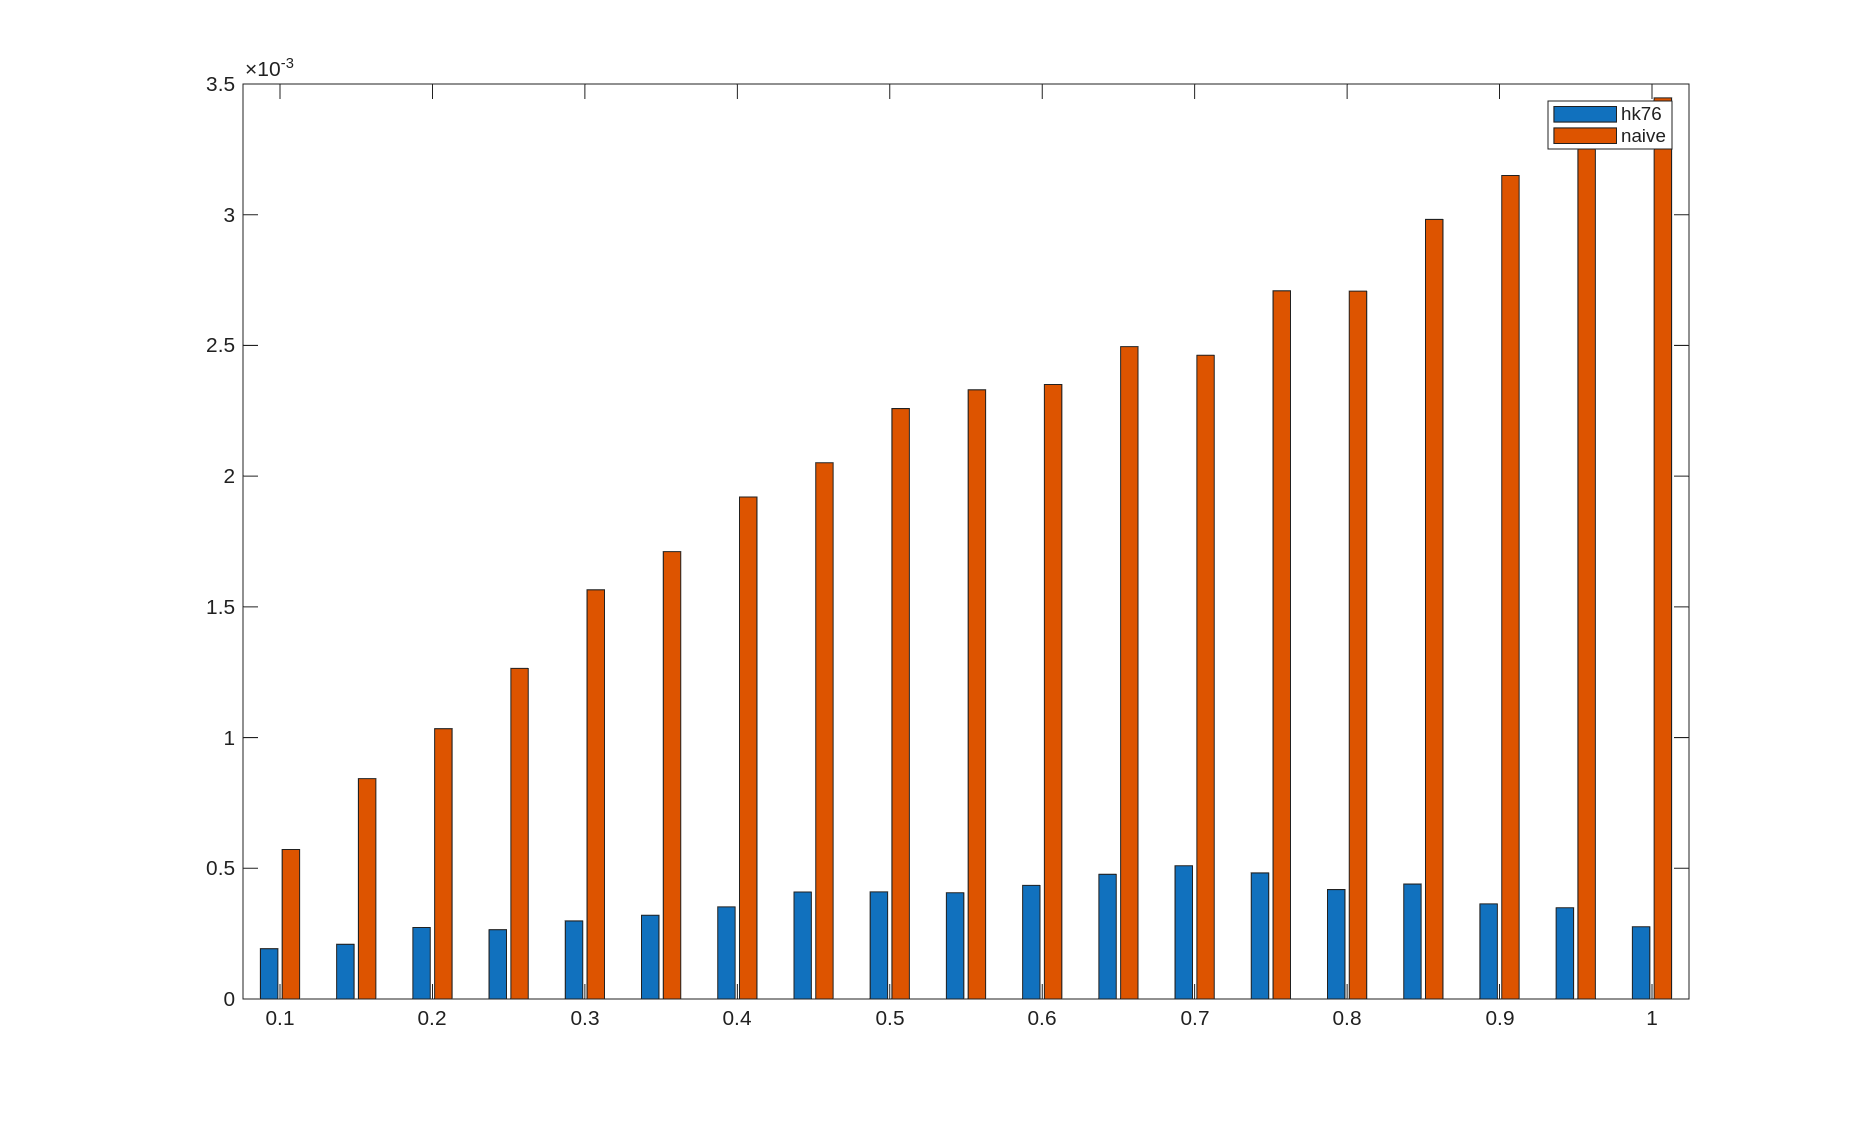
\includegraphics[width=0.85\linewidth]{images/compare_p}
	\caption{Tempo di esecuzione in funzione della probabilità di colorazione per gli algoritmi HK76 e naive.}
	\label{fig:comparep}
\end{figure}

\noindent
La Figura \ref{fig:comparep}, che mostra i tempi medi di esecuzione su $50$ iterazioni per ogni esperimento, evidenzia come l’algoritmo HK76 risulti più efficiente rispetto alla versione naive. 
\\\\
\noindent
Di seguito sono riportati i tempi medi di esecuzione:

\vspace{15px}
\noindent
\begin{tabular}{|c|*{10}{c|}}
	\hline
	\textbf{hk76} &0.0032 &   0.0047 &   0.0063  &  0.0076 &   0.0087   &  0.0110   & 0.0497  &  0.0327    &0.0086    & 0.0061 \\
	\hline
	\textbf{naive} &0.0120 &   0.0242 &   0.0377   & 0.0480  &  0.0544 &   0.0600  &  0.0643  &  0.0688 &   0.0762 &   0.0845
	\\
	\hline
\end{tabular}

\vspace{15px}
\noindent
e i relativi errori (da moltiplicare per $10^{-3}$):

\vspace{15px}
\noindent
\begin{tabular}{|c|*{10}{c|}}
	\hline
	\textbf{hk76}  & 0.0776  &  0.0643 &   0.0935 &   0.0997&    0.0864  &  0.1096   & 0.6884  &  0.4468&    0.0981  &  0.0650\\
	\hline
	\textbf{naive}  & 0.1488  &  0.2100 &   0.4623  &  0.4539 &   0.3350  &  0.4271 &   0.2585  &  0.2870 &   0.2396 &   0.3537\\
	\hline
\end{tabular}

\vspace{15px}
\noindent